\documentclass[10pt, conference]{IEEEtran}
\IEEEoverridecommandlockouts
% The preceding line is only needed to identify funding in the first footnote. If that is unneeded, please comment it out.
\usepackage{cite}
\usepackage{amsmath,amssymb,amsfonts}
\usepackage{algorithm}
% \usepackage{algorithmic}
\usepackage{algpseudocode}
\usepackage{graphicx}
\usepackage{textcomp}
\usepackage{xcolor}
\usepackage{bm}
\usepackage{subcaption}
\usepackage{float}
\usepackage{afterpage}
\usepackage[acronym]{glossaries}
\def\BibTeX{{\rm B\kern-.05em{\sc i\kern-.025em b}\kern-.08em
    T\kern-.1667em\lower.7ex\hbox{E}\kern-.125emX}}


\makeglossaries

\newacronym{ann}{ANN}{all k-nearest neighbour}
\newacronym{cews}{CEWS}{cut edges weight statistic}
\newacronym{cart}{CART}{classification and regression trees}
\newacronym{eda}{EDA}{exploratory data analysis}
\newacronym{enn}{ENN}{edited nearest neighbour}
\newacronym{fp}{FP}{false positive}
\newacronym{fn}{FN}{false negative}
\newacronym{id3}{ID3}{iterative dichotomiser 3}
\newacronym{iqr}{IQR}{Interquartile Range}
\newacronym{knn}{KNN}{k-nearest neighbours}
\newacronym{mar}{MAR}{missing at random}
\newacronym{mcar}{MCAR}{missing completely at random}
\newacronym{nan}{NaN}{not a number}
\newacronym{ni}{NI}{nonignorable}
\newacronym{renn}{RENN}{repeated edited nearest neighbour}
\newacronym{smote}{SMOTE}{synthetic minority oversampling technique}
\newacronym{tp}{TP}{true positive}
\newacronym{tn}{TN}{true negative}

\begin{document}

\title{Assignment 1 \\
Exploratory Data Analysis and the Implementation of K-Nearest Neighbor and Classification Tree Models
on Dry Bean Data
% {\footnotesize \textsuperscript{*}Note: Sub-titles are not captured in Xplore and
% should not be used}
% \thanks{Identify applicable funding agency here. If none, delete this.}
}

\author{\IEEEauthorblockN{A.D. van der Merwe}
\IEEEauthorblockA{Department of Computer Science \\
University of Stellenbosch\\
24923273 \\
24923273@sun.ac.za}
}

\maketitle

\begin{abstract}
    In this report, the application of classification algorithms is explored on the Dry Bean dataset, with a focus on
    data analysis and data preparation. The primary goal is to prepare the data and then construct two classification models,
    \acrfull{knn} and decision trees on the Dry Bean dataset and evaluate their performance on predictions of bean types.
    The characteristics of each feature and visualisation is explored to determine if there are any data quality issues.
    The data is prepared for use in the classification algorithms, which includes standardisation for \acrshort{knn} and
    post-pruning for the decision tree. K-fold cross-validation assesses the effectiveness of the model and if the
    model is deterministic, with performance measured by accuracy and F1-score. The report shows that both models can be
    tailored  to handle data quality issues and highlights the strength of each approach when beans are classified.
\end{abstract}

\section{Introduction}

Exploratory data analysis \acrshort{eda} is crucial for machine learning as it provides knowledge about the dataset and how to
approach the task at hand. More knowledge of a dataset can help make a decision on which modeling techniques to apply to the
dataset.

The approach began with a thorough characterisation of the Dry Bean dataset, to better understand the nature and distributions
of the features by the calculation of descriptive statistics. Data quality issues are identified such as missing values,
class imbalances and outliers. Data preparation techniques are applied to the data data quality issues to ensure optimal
performance of the classification algorithms that are implemented. The classification algorithms implemented are a
\acrfull{knn} and decision tree classification algorithm. For \acrshort{knn}, feature standardisation and parameter
tuning is conducted to enhance the performance of the classification model, while, for the decision tree classification model,
tree induction and post-pruning techniques are applied to prevent overfitting. To evaluate these models k-fold cross-validation
is applied and different performance features like accuracy and F1-score is used. This comprehensive approach aims to ensure
a good understanding of the dataset, analyse the data, adress any data quality issues, and determine the most effective
classification model for the Dry Bean dataset.

The rest of this paper is structured as follows: Section \ref{section:Background} provides background information on
data quality issues, data preparation techniques, \acrshort{knn} classification algorithms and decision tree classification algorithms.
Section \ref{section: Methodology} provides the methodology used to analyse and prepare the Dry Bean dataset and to build a
\acrshort{knn} and decision tree classification algorithm on the data. The empirical procedure is given in Section
\ref{section:Empirical Procedure} and the research results is given in Section \ref{section:Research Results}

\section{Background} \label{section:Background}

This section presents background information on \acrshort{eda} and techniques used to clean and transform data
for analysis or to construct models. Additionally, information on the C4.5 decision tree and k-nearest neighbours
classification models.

\subsection{Exploratory Data Analysis}\label{EDA_background}

Exploratory data analysis \acrshort{eda} first introduced by John Tukey in 1977 \cite{EDA_ref}. Tukey
emphasised that there are three key strategies in data analysis, namely:
\begin{itemize}
    \item Grapical presentation: the use of visual tools, such as plots, to explore, analyse and understand data.
    \item Flexibility in viewpoint and facilities: encourages creative and diverse approaches to analyse data
          that allows for dynamic perspective and adaptive tools.
    \item Search for parsemony and simplicity: To find simple and clear explanations in the data while
          unnecessary complexity is avoided.
\end{itemize}

\subsubsection{Data Quality Issues}

\paragraph{Missing values}

The absence of data in a dataset where a value should be present is known as a missing value. There are
three types of missing values, namely \acrfull{mar}, \acrfull{mcar} and \acrfull{ni} missing values \cite{Missing_ref}.

\acrshort{mcar} refers to a situation where missing values are distributed randomly throughout the dataset, independent
of both observed and unobserved data. Under \acrshort{mcar}, modern methods such as missing value imputation can be
used and still produce unbiased estimates, though some uncertainty is introduced. When modern methods are used
to handel \acrshort{mcar} missing values, the statistical power reduces compared to complete data.

A missing value is \acrshort{mar} if the likelihood of the missing data on the variable is unrelated to the value of
that variable itself, once other variables are taken into account. These other features help explain why data may
be missing and is known as mechanisms. Some common mechanisms include factors like education, income or age.
The \acrshort{mar} assumption holds if the pattern of missingness is random when explained by the mechanisms.

If data is missing in a systematic way and can neither be classified as \acrshort{mar} or \acrshort{mcar}, then
is the missing value classified as \acrshort{ni}. To model this type of data is complex.

There are three ways to deal with these missing values. The first option explored is to use machine learning
algorithms that is robust to missing values. The second option is to remove the instances that contains the
missing values. This option does run the risk of valuable information that may be lossed. The third option
is to impute the missing values.

When a missing value is imputed from a categorical feature, the most frequently occuring value, known as the mode,
is commonly used. When a numerical feature is imputed, the median is typically used when the data contains outliers
and the mean is used when the data contains no outliers. 

\paragraph{Outliers}

When one or more variables, of an instance in the dataset, have values that significantly differ from the overall distribution
of the data, it is known as an outlier. There are two types of outliers, namely invalid outliers that is data points included
in the dataset due to errors, and valid outliers that is correct values that are legitimately different from the rest
of the data.

There are three techniques to cope with outliers. The first technique is to remove the outliers using statistical
techniques. The second technique is to keep the outliers and apply robust estimators that are less sensitive to the
influence of the outliers. Alternatively, clipping can be performed to the outliers to limit the range of the outliers
or to impute a value to replace the outlier with. The third technique is to remove the outliers directly within the
machine learning process by the use of algorithms designed to be robust to outliers.

One approach to perform outlier detection is by the use of a statistical method known as the \acrfull{iqr} method.
The equation to calculated the \acrshort{iqr} of an input feature $\boldsymbol{\textbf{p}}$, is as follows:
\begin{equation}
    IQR^{\boldsymbol{\textbf{p}}} = Q_3^{\boldsymbol{\textbf{p}}} - Q_1^{\boldsymbol{\textbf{p}}} \label{IQR}
\end{equation}
where $Q_1^{\boldsymbol{\textbf{p}}}$ and $Q_3^{\boldsymbol{\textbf{p}}}$ is the first and third quartile of the input
feature ${\boldsymbol{\textbf{p}}}$ respectively. The equations to determine if an instance of ${\boldsymbol{\textbf{p}}}$
is an outlier, is as follows:
\begin{equation}
    \boldsymbol{\textbf{p}}_i < Q_1^{\boldsymbol{\textbf{p}}} - 1.5 \times IQR^{\boldsymbol{\textbf{p}}} \label{outlier_smaller}
\end{equation}
or if:
\begin{equation}
    \boldsymbol{\textbf{p}}_i > Q_3^{\boldsymbol{\textbf{p}}} + 1.5 \times IQR^{\boldsymbol{\textbf{p}}} \label{outlier_larger}
\end{equation}
where $\boldsymbol{\textbf{p}}_i$ is the $i$-th instance of the input feature ${\boldsymbol{\textbf{p}}}$.

Another technique to apply outlier detection is by using visual methods such as a boxplot, that displays the
distribution of data based on quartiles and highlights potential outliers, or by using a scatter plot to visualise
the the relationship between two features and can reveal outliers as points that deviate significantly from the
overall pattern.

\paragraph{Noise}

Noise refers to random or irrelevant variations in the data that can obscure patterns. There is two types of noise.
The first typeof noise is stochastic noise, with random variation in data values, a zero mean in the variation and
small deviations. If the deviation of stochastic noise is large, the feature becomes irrelevant. The second type
of noise is systematic noise, where all values shifted in a particular direction, such as due to poorly calibrated
instruments.

When handeling noise, systematic noise can be corrected by use of a few different techniques. One technique is to
make use of standardisation. Stochastic noise is handled by the machine learning process, but caution should be
used as if noise is present and the model is too complex, the model will overfit.

There are a few techniques used to remove noise in the dataset, namely \acrfull{enn}, \acrfull{renn}, \acrfull{ann},
\acrfull{cews} and Tomek links. A Tomek link is a pair of data instances $\boldsymbol{\textbf{a}}$ and
$\boldsymbol{\textbf{b}}$ where there exists a third instance $\boldsymbol{\textbf{c}}$ such that:
\begin{equation}
    d(\boldsymbol{\textbf{a}}, \boldsymbol{\textbf{c}}) \leq d(\boldsymbol{\textbf{a}}, \boldsymbol{\textbf{b}}) \label{tomek_1}
\end{equation}
or
\begin{equation}
    d(\boldsymbol{\textbf{b}}, \boldsymbol{\textbf{c}}) \leq d(\boldsymbol{\textbf{a}}, \boldsymbol{\textbf{b}}) \label{tomek_2}
\end{equation}
where $d$ is the distance between the two instances.

If $\boldsymbol{\textbf{a}}$ and $\boldsymbol{\textbf{b}}$ forma Tomek link, then either one of them is noise
or both are borderline cases. In such cases both $\boldsymbol{\textbf{a}}$ and $\boldsymbol{\textbf{b}}$
is removed to improve the quality of the dataset.

\paragraph{Imbalanced class data}

A dataset is refered to as imbalanced, if the target feature has significantly unequal
representation among its different categories. A few approaches to handel imbalanced classes are, do to
nothing, but this is not a great solution, as the train and test accuracy of the majority class may be
very good and the train and test accuracy of the minority class will be bad. Another approach to
handel imbalanced classes is to balance the training set by either the use of \acrfull{smote}
to oversample the minority class or the use of Tomek links to undersampl the majority class.

By using Tomek links as described in Equation \eqref{tomek_1} and Equation \eqref{tomek_2}, it is possible
to obtain Tomek links between classes and to then remove the majority class from each Tomek link.

\acrshort{smote} is used to oversample the minority class. The process of \acrshort{smote} is to
firstly ignore the majority class. The next step is to choose the \acrshort{knn} for each minority
instance. \acrshort{smote} then produces new instances halfway between the the instance and the
neighbours.

\subsubsection{Data Preparation}

\paragraph{Data type transformations}

Different machine learning algorithms have varying requirements for the types of input data. This necessitates
the conversion of the data from one type to another.

Discretisation is the process of converting continuous features to discrete features by the creation of bins
that group the continuous values into distinct categories. Each bin represents a specific range derived from the
the original continuous features. There is a general trade-off when a decision has to be made about the number of
bins to use. This trade off is that valuable information may be lossed, if the number of bins is very low and
if the number of bins is high, there might be very few instances in each bin or a bin could end up being empty.

There are typically two methods to encode discrete feature as a numerical Feature. The first method is known as
ordinal encoding. Ordinal encoding transforms discrete features that typically has a natural order into continuous
features. An example of this is that if the unique values of a discrete feature is cold, mild and high will be
encoded as 0, 1 and 2 respectively.

One hot encoding is typically used when there is no natural order of the unique values of the discrete feature.
If the unique values are cloudy, sunny and rainy, the values will be encoded as 1 0 0 for cloudy, 0 1 0 for
sunny and 0 0 1 for rainy.


\paragraph{Feature selection} \label{feature_selection background}

The goal of any feature selection method is to find the smallest subset of informative features that
preserves the overall performance of the model. A smaller subset of features is beneficial as the
models fitted to the data will be simpler. The smaller set of features will also produce shorter
train times and produce less overfitted models, therefore improving the generalisation of a model.

If the subset of features contains too few features, the model may underfit due to the lack of
discriminant power to differentiate between classes. An underfitted model leads to more false
positives and false negatives. Too many features in the new subset of features can introduce
noise in the training data, causing the model to overfit and increase computational complexity.

There are four types of different descriptive features to distinguish from, namely:
\begin{itemize}
    \item \textbf{Predictive} descriptive feature that provides useful information.
    \item \textbf{Interacting} descriptive feature is not informative about the target feature on its own,
          but can provide valuable information when combined with one or more other features.
    \item \textbf{Redundant} descriptive feature that has a strong correlation with another feature.
    \item \textbf{Irrelevant} descriptive feature that does not provide any useful information when a value
           is estimated for the target feature.
\end{itemize}
Ideally, after a feature selection approach is applied, will the subset of features include the predictive and
interacting features while the irrelevant and redundant features are excluded.

There are three methods to perform subset selection on a dataset, namely filter methods, wrapper methods and
embedded methods. Filter methods performs statistical tests between input feature and target feature to
identify a subset of features that are more relevant than others. The statistical test to apply types
of input features to a specific type of target feature is represented by Table \ref{tab:feature_selection_table}.
\begin{table}[h!]
    \caption{Statistical Tests for Evaluating Different Types of Input Features Against a Specific Type of Target Feature}
    \begin{center}
        \begin{tabular}{|c||c|c|}
            \hline
            \textbf{Feature}&\multicolumn{2}{|c|}{\textbf{Target Feature Type}} \\
            \cline{2-3} 
            \textbf{Type} & \textbf{\textit{Continuous}}& \textbf{\textit{Categorical}} \\
            \hline
            \textbf{\textit{Continuous}}& Pearson Correlation& LDA\\
            \hline
            \textbf{\textit{Categorical}}& Anova & Chi-Square\\
            \hline
            % \multicolumn{3}{l}{$^{\mathrm{a}}$Sample of a Table footnote.}
        \end{tabular}
        \label{tab:feature_selection_table}
    \end{center}
\end{table}

Two common approaches to apply the wrapper feature selection technique is by the use of forward and backward
feature selection that produces a best subset of features to train the model on. In forward and backward feature
selection a feature is added or removed to the best subset of features respectively and then the performance
of the model is compared when using the best subset of features and the best subset of features that has been
modified.

Embedded subset selection techniques is when an algorithm has a build in feature to perform subset selection.
Models like decision trees prune away splits on features that has little to no predictive power and techniques
like regularisation is applied to the objective function of a model to reduce the predictive
power of features that has little to no influence when predicting a target feature.

\paragraph{Normalisation}

Normalisation or scaling of input features is required for some machine learning algorithms. Normalisation
is typically required if the ranges of values for different input features differ in order of magnitudes 
and where the algorithm makes use of a distance based metric to generate classification
models. Normalisation is also used when the minimum and maximum values are not known, to
reduce the effect of outliers or to transform a range of values to a different range of values. One method
of normalisation typically used is the Z-score normalisation also known as standardisation. The equation to
perform standardisation is as follows:
\begin{equation}
    Z_{i,j} = \frac{x_{i,j} - \mu_j}{\sigma_j} \label{standardisation}
\end{equation}
where $x_{i,j}$ is the data value of the $j$-th feature for the $i$-th observation, $\mu_j$ and $\sigma_j$
is the mean and standard deviation of the $j$-th feature across all observations respectively and $Z_{i,j}$
is the Z-score of the data value at the $i$-th observation and the $j$-th feature.

Standardisation transform all of the values of each feature to have a zero-mean and a unit variance.

\subsection{K-Nearest Neighbours}\label{KNN_background}

The \acrshort{knn} algorithm was first propsed by Evelyn Fix and Joseph Hodges in 1951 \cite{KNN_ref}
in a technical report that was never published. The report contained pioneering work on nonparametric
discriminant analysis and probability density estimation and laid the foundational principles for
the \acrshort{knn} algorithm.

\acrshort{knn} is a type of instance-based learning that does not build a model based on the training
dataset. Instead, \acrshort{knn} computes the distance between the instances in the test set and all
of the instances in the training set to identify the nearest neighbours for each entry in the test set.
\acrshort{knn} relies heavily on the distance metric in order to identify the instances in the training
set closest to each of the test instances. The distance metric plays a crucial role in order to determine
the similarity between data points, that directly influences the performance and accuracy of the algorithm.
The most common distance metrics used in the \acrshort{knn} algorithm is the:
\begin{itemize}
    \item Euclidean distance metric
    \item Manhattan distance metric
    \item Minkowski distance metric
\end{itemize}

The Euclidian distance metric equation is defined as follows:
\begin{equation}
    d(\boldsymbol{\textbf{x}}_1, \boldsymbol{\textbf{x}}_2) = \sqrt{\sum_{n=1}^{N}(x_{1n} - x_{2n})^2} \label{euclidian}
\end{equation}
The Manhattan distance metric equation is defined as follows:
\begin{equation}
    d(\boldsymbol{\textbf{x}}_1, \boldsymbol{\textbf{x}}_2) = \sum_{n=1}^{N} \left| x_{1n} - x_{2n} \right| \label{manhattan}
\end{equation}
The Minkowski distance metric equation is defined as follows:
\begin{equation}
    d(\boldsymbol{\textbf{x}}_1, \boldsymbol{\textbf{x}}_2) = \left(\sum_{n=1}^{N} \left| x_{1n} - x_{2n} \right|^p\right)^\frac{1}{p} \label{minkowski}
\end{equation}
where $\boldsymbol{\textbf{x}}_1$ and $\boldsymbol{\textbf{x}}_2$ is a vector containing all the of the features of two
distinct instances in a dataset, $d(\boldsymbol{\textbf{x}}_1, \boldsymbol{\textbf{x}}_2)$ is the distance between the two
vectors $\boldsymbol{\textbf{x}}_1$ and $\boldsymbol{\textbf{x}}_2$, $N$ denotes the dimension of the vectors 
$\boldsymbol{\textbf{x}}_1$ and $\boldsymbol{\textbf{x}}_2$ or equivalently the total number of features and $x_{1n}$ and
$x_{2n}$ is the value of the $n$-th feature of the two distinct feature vectors $\boldsymbol{\textbf{x}}_1$ and
$\boldsymbol{\textbf{x}}_2$ respectively.

After the distances between the instance from the test set is calculated against all of the instances in the training set,
a distance vector $\boldsymbol{\textbf{d}}$ is obtained. The distance vector is then sorted from smallest to largest distances
and the first $k$ distances is chosen from $\boldsymbol{\textbf{d}}$. The process to classify an unseen instance,
$\boldsymbol{\textbf{x}}$, on $k$ of the instances of the training set $D$ is described by Algorithm \ref{alg:KNN_algorithm}.
\begin{algorithm}
\caption{k-Nearest Neighbours (kNN)}
\label{alg:KNN_algorithm}
\begin{algorithmic}[1]
    \Function{kNN}{$D$, $\boldsymbol{\textbf{x}}$, $k$}
        \ForAll{$\boldsymbol{\textbf{x}}_i \in D$}
            \State $\boldsymbol{\textbf{d}}$ = \Call{distance}{$\boldsymbol{\textbf{x}}_i, \boldsymbol{\textbf{x}}$}
        \EndFor
        \State \Call{sort}{$\boldsymbol{\textbf{d}}$}
        \State $S$ = set of $k$ patterns in $D$ closest to $\boldsymbol{\textbf{x}}$
        \State Return class as majority class in $S$
    \EndFunction
\end{algorithmic}
\end{algorithm}

\subsection{C4.5 Decision Trees}\label{CT_background}

The first implementation of a decision tree algorithm was introduced by Leo Brieman \textit{et al} in 1984 and
is know as \acrfull{cart} \cite{CART_ref}. In 1986 Ross Quinlan implemented the \acrfull{id3} decision tree
algorithm, which is able to cope with noise and missing values in the data \cite{ID3_ref}. In 1993 Ross Quinlan
introduced the C4.5 decision tree algorithm, which is able to handle continuous features, imbalanced classes and
introduced post-pruning \cite{C4.5_ref}.

C4.5 generates a classification tree model that consists of:
\begin{itemize}
    \item Leaf nodes that indicates different discrete classes
    \item Decision nodes that represent tests on a feature and leads to further branches in the tree.
\end{itemize}
C4.5 is induced to overfit the training data, thus the tree classifier completely separates the classes of the
training data and leads to poor generalisation on usneen data as well as outliers and noise will be in the leaves of
the tree.

C4.5 uses entropy as a measure of impurity in a dataset with respect to the target feature. The entropy of a
dataset will be 0, if all of the classes in the dataset has the same labels. If the frequency of the
classes are all equal, then will the entropy of the dataset be equal to 1. The test on an input feature
that minimises the impurity of a dataset, or equivalently maximises the information gain, is selected as the
best possible feature to split on. The equation to calculate the entropy of a dataset is as follows:
\begin{equation}
    H(D)=-\sum_{i=1}^{M} p(y_m)log_M (p(y_m))\label{entropy}
\end{equation}
and:
\begin{equation}
    p(y_m) = \frac{freq(y_m,D)}{\left\lvert D \right\rvert }\label{class_prob} 
\end{equation}
where $D$ represents the dataset, $y_m$ is the $m$-th class, $M$ is the total number of distinct classes in the
dataset, $p(y_m)$ is the probability of a class $y_m$ occuring in $D$ and where $freq(Y_m,D)$ is the number of
times class $y_m$ occurs in D.

The equation used to calculate the entropy due to the split, follows as:
\begin{equation}
    H_x(D) = \sum_{o=1}^{O} p_o H(D_o)\label{entropy_x}
\end{equation}
and:
\begin{equation}
    p_o = \frac{\left\lvert D_o \right\rvert}{\left\lvert D \right\rvert}\label{o_prob}
\end{equation}
where $x$ is the input variable used to split $D$, $O$ is the number of outcomes for $x$, $H(D_o)$ is the copnditional entropy of dataset
$D_o$ with reference to the class distribution and where $p_o$ is the probability of outcome $o$.

The equation used to calculate the information gain if $D$ is partitioned on $x$, follows as:
\begin{equation}
    gain(x) = H(D) - H_x(D)\label{info_gain}
\end{equation}
The information gain calculation favours input features with many outcomes and introduces bias as the tree
creates multiple branches, one for each unique value. The solution to the bias is to normalise the information gain with entropy
with respect to test outcomes. The equation for the gain ratio is as follows:
\begin{equation}
    gainRatio(x) = (1-F)\frac{gain(x)}{splitInfo(x)}\label{gainRatio}
\end{equation}
and:
\begin{equation}
    splitInfo(x) = -\sum_{o=1}^{O}p_o log_O(p_o)\label{splitInfo}
\end{equation}
where $F$ is the fraction of patterns in $D$ for which the value of $x$ is missing.
The objective of the tree is to select $x$ that maximise the gain ratio.

In order to handel numerical continuous features, C4.5 first sorts the number of unique values, denoted by $I$,
found in the numeric input feature $x$ to create the sequence, $(v_1,v_2,...,v_I)$ ordered from smallest to largest.
C4.5 performs $I$-1 splits between $v_i$ and $v_{i+1}$ and for each of these splits the information gain is calculated by use of
Equation \eqref{gainRatio}. The split with the highest calculated information gain will be chosen and the threshold to
split the tree on is calculated as follows:
\begin{equation}
    \epsilon = \frac{v_i + v_{i+1}}{2}\label{numeric}
\end{equation}
where $\epsilon$ is the threshold to split the tree on. C4.5 then generates two decision nodes with test $x < \epsilon$ and $x >= \epsilon$.

C4.5 partitions the dataset $D$ in the absence of missing values as follows: 
\begin{equation}
    w_j(D_o) = 1, w_j(D_q)=0, \forall q \neq o \label{no_missing}
\end{equation}
where each pattern $j$ in $D$ belongs to subset $D_o$ with weight $w_i(D_o)$, provided that pattern $j$ no missing value for the input
feature $x$. If pattern $j$ has a missing value for feature $x$, it is assigned to all outcomes with a weight given by:
\begin{equation}
    w_j(D_o) = w_j(D)p_o \label{with_missing}
\end{equation}
where the probability of the outcome is now calculated as follows:
\begin{equation}
    p_o = \frac{\Sigma_{x_j \epsilon D \text{ with outcome } _o} w_j(D)}{\Sigma_{x_j \epsilon D \text{ with any known outcome}} w_j(D)}
\end{equation}

To determine the optimal input feature $x$ to split the data on, the process follows these steps:
\begin{itemize}
    \item Calculate the entropy of the current dataset, $H(D)$ by use of Equation \eqref{entropy}
    \item Compute the conditional entropy for each input feature $x$, $H_x(D)$ by use of Equation \eqref{entropy_x}
    \item Calculate the information gain for each feature if $D$ would be split on $x$ by use of Equation \eqref{info_gain}
    \item Using the calculated information gain, calculate the gain ratio by use of Equation \eqref{gainRatio}
    \item Select the feature with the highest gain ratio and split $D$ into $O$ subsets
    \item Repeat the process on each subset until the tree has been induced to completely separate the classes
\end{itemize}

Algorithm \ref{alg:CTI_algorithm} describes the process to fully induce the decision tree. 
\begin{algorithm}
    \caption{Classification Tree Induction}
    \label{alg:CTI_algorithm}
    \begin{algorithmic}[1]
        \Function{InduceTree}{$D$}
            \If{$\left\lvert D \right\rvert$ = 0}
                \State Return leaf with default class
            \EndIf
            
            \If{$\left\lvert D \right\rvert$ $>$ 0 and $\forall \boldsymbol{\textbf{x}} \in D$ the class is the same, i.e. $y_m$}
                \State Return leaf with class label $y_m$, containing $D$
            \EndIf{}

            \State Select a test based on a single input variable
            \State Split $D$ into $D_1$,$D_2$,...,$D_o$, where $O$ is the number of outcomes
            \For{$o$ = 1 to $O$}
                \State \Call{InduceTree}{$D_o$}
            \EndFor
        \EndFunction
    \end{algorithmic}
\end{algorithm}

In order to overcome the issues of the fully induced tree that overfits the training data, as well as outliers and
noise in the leaves of the tree, C4.5 introduced post-pruning. C4.5 replaces the tests in the deepest level
of the tree with leaf nodes, where the prediction of the leaf node is the class that occurs the most in the new subset.
A validation set is used to test the generalisation performance of unseen data and if the generalisation performance
increases, the tree prunes away the decision node and replaces it with the leaf node. If the generalisation performance
does not improve, the decision node is then re-inserted into the tree. This process is repeated until no more decision
nodes are replaced. The tree is now robust to outliers and noise.

\subsection{Performance Metrics} \label{performance_metric_background}

Performance metrics are essential tools when the effectiveness of classification models are evaluated. Performance metrics
provide a quantitative measure of how reliable and accurate a prediction model performs classification on a dataset.
Key metrics include accuracy, precision, recall, and F1-score, each offering unique insights into different aspects
of model performance \cite{Performance_ref}.

\paragraph{Accuracy}
Accuracy is a common method used to evaluate the performance of classification models. The accuracy of
a predictive classification model is determined by the proportion of correctly predicted labels against
the total number of predictions. The calculation of the accuracy of a predictive model is as follows:
\begin{equation}
    \text{Accuracy} = \frac{\text{Number of Correct Predictions}}{\text{Total Number of Predictions}} \label{accuracy}
\end{equation}

Accuracy is a popular choice of performance measure mainly beacause it is fairly easy to understand and compute.
Accuracy generally perform well on well balanced datasets. On imbalanced datasets, accuracy can produce
values that are misleading. If a model predicts 

\paragraph{Precision and Recall}
Precision is the proportion of \acrfull{tp} predictions against all of the \acrshort{tp} and \acrfull{fp}.
The equation to calculate the precision of a classification model is as follows:
\begin{equation}
    \text{Precision} = \frac{\text{True Positives}}{\text{True Positives} + \text{False Positives}} \label{Precision}
\end{equation}

Recall is the proportion of \acrshort{tp} predictions against all of the \acrshort{tp} and \acrfull{fn}.
The equation to calculate the recall of a classification model is as follows:
\begin{equation}
    \text{Recall} = \frac{\text{True Positives}}{\text{True Positives} + \text{False Negatives}} \label{Recall}
\end{equation}

\paragraph{F1-score}

The F1-score, also known as the Dice similarity coefficient, is the harmonic mean of precision and recall,
that provides a balance between the precision and recall \cite{F1-score_ref}.
In multiclass classificationprecision and recall are adapted from binary classification to handle multiple classes.
Instead of focusing on a single positive and negative class, these metrics are calculated for each class,
where each class is treated as the positive class while considering all others as negative. The F1-score
is calculated for each clas and then averaged. There are three types of averaging F1-score metrics.

The first F1-score metric is the macro averaging F1-score, where the F1-score is calculated  independently for each label
and then these scores are averaged, giving each class the same weight. The equation used to calculate the macro F1-score is
as follow:
\begin{equation}
    F1_{macro} = \frac{1}{C} \sum_{i=1}^{C} \frac{2 \times Precision_i \times Recall_i}{Precision_i + Recall_i} \label{macro_F1}
\end{equation}
where $C$ is the number of classes.

The second F1-score metric used is the micro averaging F1-score, where the contributions of all of the classes
are aggregated inore to compute the total true positives, false positives and false negatives. The equation used
to calculate the micro F1-score is as follow:
\begin{equation}
    F1_{micro} = \frac{2 \times Precision_{micro} \times Recall_{micro}}{Precision_{micro} + Recall_{micro}} \label{micro_F1}
\end{equation}
Micro averaging treats each instance equally and is therefore useful when a dataset contains imbalanced classes. 

The last F1-score metric is known as the weighted averaging F1-score. The weighted F1-score computes the F1-score
for each class, just like in the macro F1-score. Each score is then weigh by the number of true instances in each class.
The equation used to calculate the weighted F1-score is as follow:
\begin{equation}
    F1_{weighted} = \sum_{i=1}^{C} w_i \frac{2 \times Precision_i \times Recall_i}{Precision_i + Recall_i} \label{weight_F1}
\end{equation}
where $w_i$ is the proportion of true instances for label $i$. The equation to calculate $w_i$ is as follows:
\begin{equation}
    w_i = \frac{TP_i + FN_i}{\sum_{j=1}^{C}(TP_j + FN_j)}    
\end{equation}
where the denominator is the sum of all the true positives and false negatives of all classes, $TP_i$ is the \acrshort{tp}
for class $i$ and $FN_i$ is the \acrshort{fn} for class $i$.

When the distribution of the classes in a dataset is imbalanced, the F1-score is considerd a more optimal performance metric
than the accuracy of a model given that the weighted F1-score, macro F1-score and micro F1-score considers both false positives
and false negatives.

\section{Methodology} \label{section: Methodology}

This section provides the approach taken to explore and analyse the dry beans dataset to identify and address data quality
issues. Additionally, it details the methodology used to classify dry bean types through the use of a \acrshort{knn}
and classification tree model.

\subsection{Data Overview} \label{Data_Overview}

The structure and characteristics of the Dry Beans dataset are thoroughly investigated. The details on the number of instances
and types of features are investigated to provide a foundational understanding for the subsequent data analysis.

The Dry Bean dataset contains 13611 instances and 22 features. Among these features, 19 are numerical features and 3 are
categorical features, with the `Class' feature being the target feature. A closer examination reveals that
missing values in the dataset are represented by `?'. Missing values identified by `?' is very problematic as it changes
the continuous features containing missing values into discrete features. The dataset is modified so that each instance
of a missing value is changed from `?' to a value of \acrfull{nan}. The next step is to identify some important
characteristics of each feature and investigate these characteristics. The important characteristics of each
continuous feature are summarised in Table \ref{tab:continuous features}.

% \clearpage
\begin{table*}[h!]
    % \caption{\textbf{Continuous Features}}
    \caption{Continuous Features}
    \begin{center}
    \begin{tabular}{|c||c|c|c|c|c|c|c|c|c|c|}
        \hline
        \textbf{Features}&\textbf{Count}&\textbf{\% Miss.}&\textbf{Card.}&\textbf{Min.}&\textbf{$1^{st}$ Qrt.}&\textbf{Mean}&\textbf{Median}&\textbf{$3^{rd}$ Qrt.}&\textbf{Max}.&\textbf{Std Dev.}\\
        \hline
        %   	                    Count   % Miss     Card.    Min         1st Q       Mean          Median      3rd Q       Max         Std Dev
        \textbf{Area}               &13611  &0.0       &12011   &20420      &36328      &53048.2845 &44652      &61332      &254616     &29324.0958\\
        \textbf{Perimeter}          &13611  &0.0       &13351   &524.736    &703.5235   &855.2835   &794.941    &977.213    &1985.37    &214.2897\\
        \textbf{MajorAxisLength}    &13611  &0.0       &13543   &183.601165 &253.303633 &320.1419   &296.883367 &376.495012 &738.860153 &85.6942\\
        \textbf{MinorAxisLength}    &13611  &0.0       &13543   &122.512653 &175.848170	&202.2707   &192.431733 &217.031741 &460.198497 &44.9701\\
        \textbf{AspectRation}       &13611  &0.0       &13543   &1.024868   &1.432307   &1.5832     &1.551124   &1.707109	  &2.430306   &0.2467\\
        \textbf{Eccentricity}       &13611  &0.0       &13543   &0.218951   &0.715928   &0.7509     &0.764441	  &0.810466	  &0.911423   &0.0920\\
        \textbf{ConvexArea}         &13611  &0.0       &12066   &-30        &36714.5    &53765.6926 &45178      &62294      &263261     &29778.0094\\
        \textbf{EquivDiameter}      &13611  &0.0       &12012   &0.161417   &215.068003 &476.2541   &238.438026 &279.452162 &3014441    &25836.8656\\
        \textbf{Extent}             &13611  &0.044082  &13529   &0.555315   &0.718641   &0.7497     &0.759874   &0.786852	  &0.866195	  &0.0491\\
        \textbf{Solidity}           &13611  &0.0       &13526   &0.919246	&0.985670	&0.9871     &0.988283   &0.990013   &0.994677   &0.0047	\\
        \textbf{Roundness}          &13611  &0.0       &13543   &0.489618   &0.832096   &0.8733     &0.883157   &0.916869   &0.990685   &0.0595\\
        \textbf{Compactness}        &13611  &0.132246  &13525   &0.640577	&0.762577	&0.7999	    &0.801291	  &0.834270   &0.987303   &0.0617\\
        \textbf{ShapeFactor1}       &13611  &0.0       &13543   &0.002778   &0.005900   &0.0066 	&0.006645   &0.007271   &0.010451   &0.0011\\
        \textbf{ShapeFactor2}       &13611  &0.0       &13543   &0.000564	&0.001154	&0.0017	    &0.001694	  &0.002170   &0.003665   &0.0006\\
        \textbf{ShapeFactor3}       &13611  &0.0       &13543   &0.410339   &0.581359	&0.6436     &0.642044	  &0.696006	  &0.974767   &0.0990\\
        \textbf{ShapeFactor4}       &13611  &0.0       &13611   &0.695579	&1.614151	&2.3681	  &2.368757   &3.115695	  &3.966119   &0.8716\\
        \textbf{ShapeFactor5}       &13611  &0.0       &13543   &0.947687   &0.993703   &0.9951	  &0.996386	  &0.997883   &0.999733   &0.0044\\
        \textbf{ShapeFactor6}       &13611  &0.036735  &13606   &0.000466	&45.258826	&89.3586	  &88.76667   &134.273148 &178.985023 &51.8386\\
        \textbf{Sort order}         &13611  &0.0       &13611   &0.000089   &0.248187   &0.5003     &0.50381    &0.750096   &0.999985   &0.2879\\

        \hline
    \end{tabular}
    \label{tab:continuous features}
    \end{center}
\end{table*}
The important characteristics of each discrete feature in the Dry Bean dataset is summarised in Table
\ref{tab:categorical features}.

\begin{table*}[h!]
    % \caption{\textbf{Continuous Features}}
    \caption{Categorical Features}
    \begin{center}
    \begin{tabular}{|c||c|c|c|c|c|c|c|c|c|}
        \hline
        \textbf{Features}&\textbf{Count}&\textbf{\% Miss.}&\textbf{Card.}&\textbf{Mode}&\textbf{Mode Freq.}&\textbf{Mode \%}&\textbf{$2^{nd}$ Mode}&\textbf{$2^{nd}$ Mode Freq.}&\textbf{$2^{nd}$ Mode \%}\\
        \hline
        %   	                    Count   % Miss     Card.    Mode      Mode Freq   Mode %        2nd Mode    2nd Mode Freq  2nd Mode %
        \textbf{Constantness}       &13611  &0.0       &2       &1        &12289      &90.287268     &0          &1322         &9.712732\\
        \textbf{Colour}             &13611  &0.044082  &4       &brown    &6115       &44.926897    &black      &3541          &26.015723\\
        \textbf{Class}              &13611  &0.124899  &7       &DERMASON &3542       &26.02307     &SIRA       &2634          &19.351995\\

        \hline
    \end{tabular}
    \label{tab:categorical features}
    \end{center}
\end{table*}

\begin{figure}[H]
\end{figure}
\begin{figure}[H]
\end{figure}
\begin{figure}[H]
\end{figure}
\begin{figure}[H]
\end{figure}
\begin{figure}[H]
\end{figure}
\begin{figure}[H]
\end{figure}
\begin{figure}[H]
\end{figure}
\begin{figure}[H]
\end{figure}
\begin{figure}[H]
\end{figure}

\noindent

The most important observation made from Table \ref{tab:categorical features} is that the `Class' feature
is imbalanced, as the first and second modes together form 45\% of the data. The five other classes
makes up the remaining 55\%, and thus the `Class' feature is imbalanced.

Several points of interest emerge after a closer examination of Table \ref{tab:continuous features}. The first
observation made is that the feature `Sort Order' feature has a cardinality of 13611, a minimum of approximately 0,
a first quartile value of approximately 0.25, a mean of approximately 0.5, a third quartile of approximately 0.75 and
a maximum value of approximately 1. These statistics all indicate that `Sort Order' is a unique identifier or index.
As a result, `Sort Order' may be considered as an irrelevant feature for predictive modeling purpose.

The second observation made is that feature `ConvexArea' contains a negative number as the minimum value. This is
impossible as area can not be negative. The boxplot of feature `ConvexArea' is given by Figure
\ref{ConvexArea_boxplot_negative} to further investigate the properties of the feature `ConvexArea'.
\begin{figure}[h!]
    \centerline{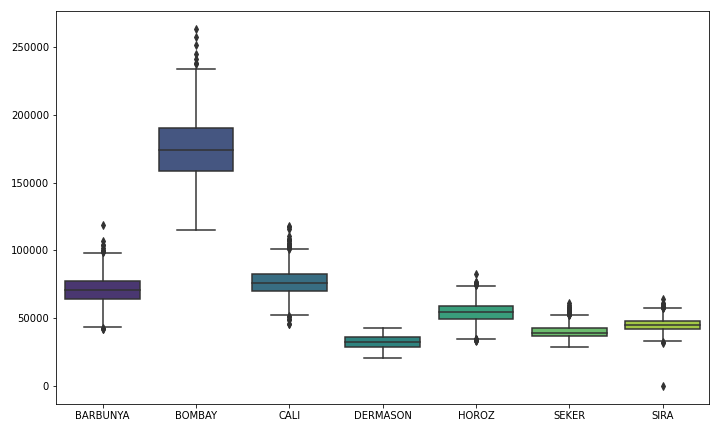
\includegraphics[scale=0.35]{../Plots/Negative ConvexArea boxplot.png}}
    \caption{Boxplot of feature ConvexArea vs feature Class}
    \label{ConvexArea_boxplot_negative}
\end{figure}

Figure \ref{ConvexArea_boxplot_negative} clearly shows that the negative value is an obscure outlier, thus can this
instance of the dataset be classified as an invalid outlier and should either be imputed or dropped from the dataset.


The third observation made is that both the minimum and the maximum values of feature `EquivDiameter' deviates
largely from the rest of the statistics. This large deviation may indicate that these instances of the dataset
are also invalid outliers. Figure \ref{EquivDiameter boxplot before} is the boxplot of feature `EquivDiameter'
that helps to investigate the obscure values of the instances in the dataset.
\begin{figure}[H]
    \centerline{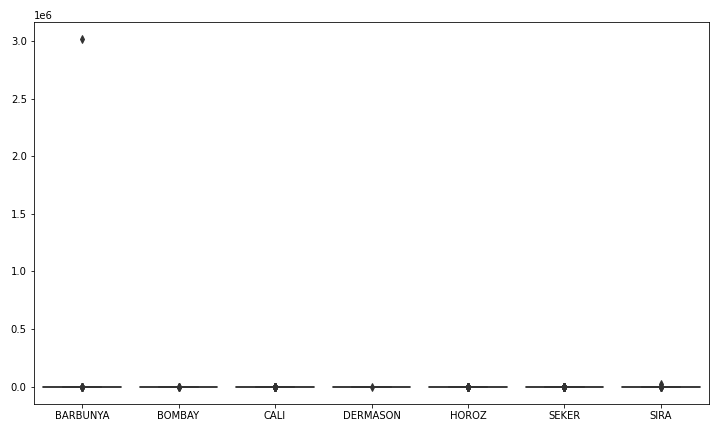
\includegraphics[scale=0.35]{../Plots/EquivDiameter outlier boxplot.png}}
    \caption{Boxplot of feature EquivDiameter vs feature Class}
    \label{EquivDiameter boxplot before}
\end{figure}

From Figure \ref{EquivDiameter boxplot before} it is quite clear that the maximum value of feature `EquivDiameter'
is an invalid outlier. This instance is dropped from the dataset and the boxplot is generated again, as shown
in Figure \ref{EquivDiameter boxplot before 2}, to investigate the minimum value of the feature `EquivDiameter'.
\begin{figure}[H]
    \centerline{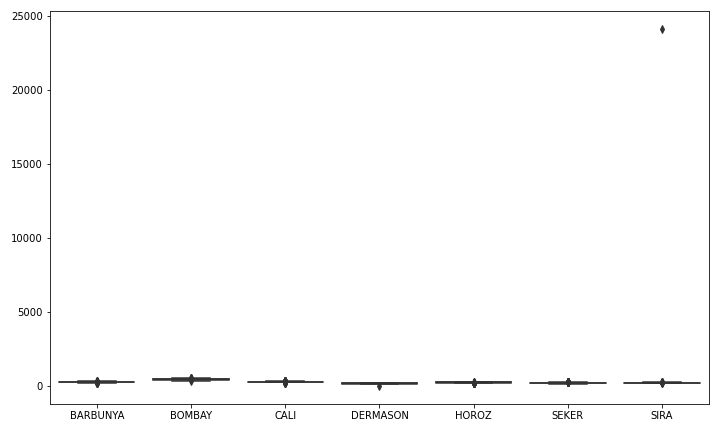
\includegraphics[scale=0.35]{../Plots/EquivDiameter outlier boxplot 2.png}}
    \caption{Boxplot of feature EquivDiameter vs feature Class after the maximum value was dropped}
    \label{EquivDiameter boxplot before 2}
\end{figure}

As seen in Figure \ref{EquivDiameter boxplot before 2} there is another instance in the dataset that deviates
significantly from the rest of the observations and can also be classified as an invalid outlier. This outlier
is also removed from the dataset and the boxplot is again generated, as shown in Figure
\ref{EquivDiameter boxplot before 3}, to investigate the minimum value of the feature `EquivDiameter'.
\begin{figure}[H]
    \centerline{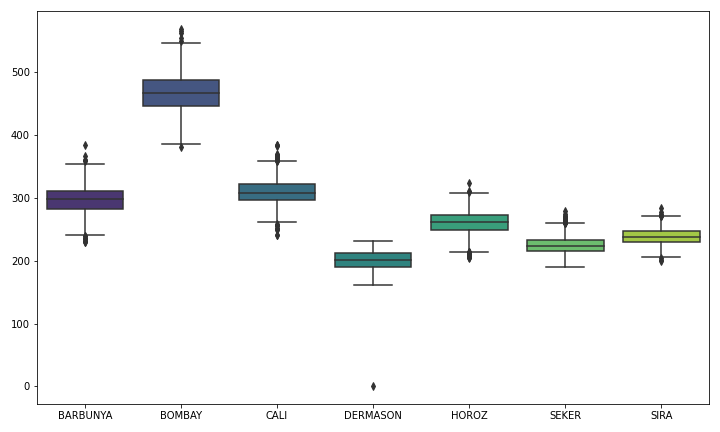
\includegraphics[scale=0.35]{../Plots/EquivDiameter outlier boxplot 3.png}}
    \caption{Boxplot of feature EquivDiameter vs feature Class after the invalid outliers were dropped}
    \label{EquivDiameter boxplot before 3}
\end{figure}

From Figure \ref{EquivDiameter boxplot before 3} it is clear that the minimum value is also an invalid outlier
that should either be imputed or removed from the dataset.

\subsection{K-Nearest Neighbours}

\paragraph{Data preparation}

Data preparation is a very crucial step that must be completed before the \acrshort{knn} algorithm can be applied to the Dry
Bean dataset. If a \acrshort{knn} model is implemented as described in Section \ref{KNN_background}, then
will the \acrshort{knn} model be robust to missing values, noise and outliers in the dataset. To prepare
the Dry Bean dataset for a \acrshort{knn} model, the missing values have to be replaced with \acrshort{nan}
and the insatnces that contains missing values in the `Class' feature is dropped.

\acrshort{knn} is an instance-based learning algorithm that calculates the distance between feature
instances to classify new data points based on the majority class of their nearest neighbours. Therefore, all features need
to be numeric for the distance calculations to be valid. The `Colour' feature is a categorical feature with no
natural ordering and will therefore be one hot encoded.

This implementation of \acrshort{knn} is sensitive to imbalanced classes. The `Class' feature is imbalanced, as
discussed in Section \ref{Data_Overview}. Tomek links and \acrshort{smote} resampling techniques are applied to the
dataset in order to address this imbalance and improve the performance of the \acrshort{knn} classification model.
Additionally, standardisation is applied to scale the feature values, to ensure that all features contribute
equally to the distance calculations and to enhance the accuracy of the model. Standardisation is applied
by the use of Equation \eqref{standardisation}.

Subset feature selection has to be applied to the newly resampled and standardised dataset. If a \acrshort{knn} algorithm
is fitted with all of the input features, it becomes very likely that the algorithm overfits, thus having a poor
generalisation on unseen data. In Section \ref{feature_selection background}, feature selection is discussed in detail.
By the use of a wrapper feature selection technique, the dimension of the Dry Bean dataset can be reduced to the
construction of a \acrshort{knn} algorithm that overfits the dataset.

\paragraph{\acrshort{knn} model implementation}

The \acrshort{knn} model for predictive analysis on the Dry Bean dataset is implimented as described
in Section \ref{KNN_background}. An additional integer control parameter has been introduced to
Algorithm \ref{alg:KNN_algorithm} that allows for the selection of the appropriate distance metric
to be applied in the process of model execution. The implementation of the \acrshort{knn} model is represent
by Algorithm \ref{alg:KNN_improved_algorithm}
\begin{algorithm}
    \caption{Improved k-Nearest Neighbours (kNN)}
    \label{alg:KNN_improved_algorithm}
    \begin{algorithmic}[1]
        \Function{kNN}{$D$, $\boldsymbol{\textbf{x}}$, $k$, $p$}
            \ForAll{$\boldsymbol{\textbf{x}}_i \in D$}
                \State $\boldsymbol{\textbf{d}}$ = \Call{distance}{$\boldsymbol{\textbf{x}}_i, \boldsymbol{\textbf{x}}$, $p$}
            \EndFor
            \State \Call{sort}{$\boldsymbol{\textbf{d}}$}
            \State $S$ = set of $k$ patterns in $D$ closest to $\boldsymbol{\textbf{x}}$
            \State Return class as majority class in $S$
        \EndFunction
    \end{algorithmic}
\end{algorithm}

where the equation to calculate the distance between two input features of instances
$\boldsymbol{\textbf{x}}_1$ and $\boldsymbol{\textbf{x}}_2$ is as follows:
\begin{equation}
    d(\boldsymbol{\textbf{x}}_1, \boldsymbol{\textbf{x}}_2) = \left(\sum_{n=1}^{N} \left| x_{1n} - x_{2n} \right|^p\right)^\frac{1}{p} \label{p_distance}
\end{equation}

The Equation \eqref{p_distance} is observed to be the Minkowski distance metric. If $p$ is equal to one, the Manhattan
distance is calculated between $\boldsymbol{\textbf{x}}_1$ and $\boldsymbol{\textbf{x}}_2$. If $p$ is equal to two,
the Euclidean distance is calculated between $\boldsymbol{\textbf{x}}_1$ and $\boldsymbol{\textbf{x}}_2$ and if
p is larger than 2, the Minkowski distance is calculated between $\boldsymbol{\textbf{x}}_1$ and $\boldsymbol{\textbf{x}}_2$.

\subsection{Classification Tree}

\paragraph{Data preparation}

Data preparation is a crucial step that must be completed before the classification tree algorithm can be applied to the
Dry Bean dataset. If a classification tree algorithm is implemented as described in \ref{CT_background}, then will
the classification tree be robust to outliers, missing values and noise in the dataset.
To prepare the Dry Bean dataset for a classification tree model, the missing values have to be replaced
with \acrshort{nan} and the insatnces that contains missing values in the `Class' feature is dropped. The
classification tree is sensitive to class imbalances. Instead of resampling the data, another technique is implemented
within the classification tree algorithm to enhance the algorithms robustness to class imbalances.

\paragraph{Classification Tree model implementation}

The classification tree model for predictive analysis on the Dry Bean dataset is implimented as described
in Section \ref{CT_background}. The inclusion of these two additional control parameters, being the maximum depth of the tree
and the minimum number of samples needed to create a split in the tree, creates a tree that is less prone to
overfitting. In Algorithm \ref{alg:CTI_imporved_algorithm} the two additional control parameters are added.
\begin{algorithm}[H]
    \caption{Improved Classification Tree Induction}
    \label{alg:CTI_imporved_algorithm}
    \begin{algorithmic}[1]
        \Function{InduceTree}{$D$, $depth$}
            \If{$\left\lvert D \right\rvert$ = 0}
                \State Return leaf with default class
            \EndIf
            
            \If{$\left\lvert D \right\rvert$ $<$ \text{min\_sample\_split} or $depth$ $>=$ $max depth$}
                \State Return leaf with class label $y_m$, containing $D$
            \EndIf

            \If{$\left\lvert D \right\rvert$ $>$ 0 and $\forall \boldsymbol{\textbf{x}} \in D$ the class is the same, i.e. $y_m$}
                \State Return leaf with class label $y_m$, containing $D$
            \EndIf

            \State Select a test based on a single input variable
            \State Split $D$ into $D_1$,$D_2$,...,$D_o$, where $O$ is the number of outcomes
            \For{$o$ = 1 to $O$}
                \State \Call{InduceTree}{$D_o$, $depth+1$}
            \EndFor
        \EndFunction
    \end{algorithmic}
\end{algorithm}

An additional return condition was added to reduce the complexity of the model and to create a
classification tree that is less prone to overfit. If the current depth $depth$
is greater than or equal to the maximum depth control parameter, or if the sample size is smaller
than the minimum sample split, the tree returns the majority class in the data.

The classification tree makes use of pruning by seperating the training set into a training
and validation set. The tree is induced by the use of training set and then pruned by use of the
validation set. Algorithm \ref{alg:prune_tree_simplified} explains the algorithm used to 
prune the tree. 
\begin{algorithm}[H]
    \caption{Simplified Post-Pruning of a Decision Tree}
    \label{alg:prune_tree_simplified}
    \begin{algorithmic}[1]
        \Function{PruneTree}{$X_{\text{val}}$, $y_{\text{val}}$}
            \If{Tree is not trained}
                \State \textbf{raise} ValueError("The tree has not been trained yet.")
            \EndIf
            \State \Call{PruneNode}{root, $X_{\text{val}}$, $y_{\text{val}}$}
        \EndFunction

        \Function{PruneNode}{node, $X_{\text{val}}$, $y_{\text{val}}$}
            \If{node is a leaf}
                \Return
            \EndIf
            
            \For{each branch in node.branches}
                \State Determine threshold and mask for $X_{\text{val}}$ based on the branch value.
                \State Subset $X_{\text{val}}$ and $y_{\text{val}}$ using the mask.
                \If{the subset is not empty}
                    \State \Call{PruneNode}{branch, $X_{\text{val\_subset}}$, $y_{\text{val\_subset}}$}
                \EndIf
            \EndFor
            
            \If{$X_{\text{val}}$ is not empty}
                \State Compute original predictions and original F1-score.
                \State Temporarily make the node a leaf and set the prediction to the majority class.
                \State Compute pruned predictions and pruned F1-score.
                \If{pruned F1-score $<$ original F1-score}
                    \State Revert node to its original state.
                \EndIf
            \EndIf
        \EndFunction
    \end{algorithmic}
\end{algorithm}

F1-score is used as the performance metric to compare the predictions of the original tree to the
predictions of the pruned tree. If the F1-score of the pruned tree is lower than the F1-score
of the original tree, the changes are reverted to ensure that pruning does not degrade the performance
of the model.

\section{Empirical Procedure} \label{section:Empirical Procedure}

\subsection{Performance Metrics}

Accuracy is used to evaluate the performance of the \acrshort{knn} model, as the dataset has been
resampled to have balanced class distributions. As for the Classification tree, the performance
measures used to evaluate the model will be the weighted F1-score, since the dataset has an
imbalanced class distribution.

\subsection{Control Parameters}

The \acrshort{knn} experiments are performed by the use of the euclidian distance metric and a value of
147 for k. The experiments of the classification tree are performed by the use of a max depth of 9 and
a minimum sample split of 2.

\subsection{Experimental Setup}

To evaluate the performance of both the \acrshort{knn} and classification tree algorithms, a 5-fold cross
validation technique was applied, that splitted the Dry Bean dataset into five equally distributed datasets.
Four of these datasets were used to train each model and the remaining dataset was used to test the
classification algorithm. This ensured that the evaluation was fair and consistent across the entire dataset and
the bias that might arise from relying on a single training-test split was reduced. The rotation of the test set,
allowed for a more comprehensive understanding of the performance of the model on unseen data.

\subsection{Statistical Significance and Analysis}

The statistical significance of the results from the \acrshort{knn} and classification tree models is determined
by the evaluation of the accuracy and weighted F1-score respectively of each of the models implemented by the use
of a 5-fold cross-validation over a grid of different possible values that the control parameters could be. By use of the Kruskal-Wallis
test to check for stochastic dominance amongst the samples. The paired t-test was then performed to obtain this optimal value of the
control parameters for both the \acrshort{knn} and classification tree models.

\section{Research Results} \label{section:Research Results}


\section{Conclusion} \label{section:Conclusion}

In this report, the Dry Bean dataset was thoroughly analysed and the important characteristics of each feature was investigated
to better understand the data and to identify any data quality issues. The Dry Bean dataset was used to construct two classification
models, namely a \acrfull{knn} and a decision tree. Before the \acrshort{knn} model was trained on the dataset, some data
quality issues had to be addressed such as resampling by use of Tomek links and \acrfull{smote} to balance the class distributions,
standardisation of the numerical input features and best subset selection using backwards subset selection. The \acrshort{knn}
algorithm implemented is robust to missing values, outliers and noise in the dataset. The decision tree is induced to overfit the data
and seperate the classes with 100\% accuracy and by use of post-pruning, to optimise the tree and make the model less prone to overfit.

By the use of k-fold cross-validation and performance metrics such as accuracy for the \acrshort{knn} model, because of the evenly
distributed classes and F1-score for the decision tree classification model, because of the imbalanced distributed classes,
it was shown that both classification models can effectively be applied to the Dry Bean dataset. After the implementation
of a grid search and the appropriate statistical tests, to determine the optimal values for the number of neighbours and the optimal
distace function to use, the \acrshort{knn} model produced a number of neighbours equal to 147 and the distance metric used was
the Euclidean distance metric. The optimal values for the maximum depth and minimum sample split for the decision tree after
the implementation of a grid search and the appropriate statistical tests came out to be 9 and 2 respectively.

In conclusion, both the \acrshort{knn} and decision tree models are viable methods for the task of classification on the Dry Bean dataset.
However, the model that performs better classifications on the Dry Bean dataset is the \acrshort{knn} classification model.

\begin{thebibliography}{00}
    \bibitem{Missing_ref} A. C. Acock "Working with missing values." In: Journal of Marriage and family (2005).
    \bibitem{Performance_ref} J. Braet, M. Cristina, Hinojosa-Lee, and J. Springael. "Evaluating performance metrics in emotion lexicon distillation: a focus on F1 scores." (2024).
    \bibitem{CART_ref} L. Breiman, J. Friedman, R. A. Olshen and C. J. Stone "Classification and Regression Trees." In: Routledge.  (1984).
    \bibitem{F1-score_ref} B. J. Erickson, and K. Felipe "Magician’s corner: 9. Performance metrics for machine learning models." In: Radiology: Artificial Intelligence 3, no. 3 (2021): e200126.
    \bibitem{KNN_ref} M. C. Jones, B. W. Silverman “E. Fix and J.L. Hodges (1951): An Important Contribution to Nonparametric Discriminant Analysis and Density Estimation: Commentary on Fix and Hodges (1951).” In: International Statistical Review / Revue Internationale de Statistique, vol. 57, no. 3, (1989).
    \bibitem{ID3_ref} J. R. Quinlan "Induction of decision trees" In: Mach Learn 1 (1986).
    \bibitem{C4.5_ref} J. R. Quinlan "C4. 5: programs for machine learning." In: Elsevier, (1993).
    \bibitem{EDA_ref} J. W. Tukey. "Exploratory data analysis." In: Reading/Addison-Wesley (1977).
\end{thebibliography}


\printglossary[type=\acronymtype]

\begin{table}[h!]
    \caption{Hyperparameter tuning for Classification tree}
    \begin{center}
        \begin{tabular}{|c||c|c|c|c|}
            % \hline
            % \textbf{Max depth}
            % \cline{0-5}
                        & \textbf{2} & \textbf{3} & \textbf{4} & \textbf{5} \\
            \hline
            \textbf{8}  & 94.47388 & 94.47388 & 94.47388 & 94.45916\\
            \textbf{9}  & 94.88595 & 94.86387 & 94.84180 & 94.82708\\
            \textbf{10} & 94.83444 & 94.82708 & 94.74614 & 94.78293\\
            \textbf{11} & 94.75350 & 94.73878 & 94.76821 & 94.79765\\
            \textbf{12} & 94.79029 & 94.76821 & 94.77557 & 94.67255\\
        \end{tabular}
    \end{center}
\end{table}

% \begin{figure}[b!]
%     \centerline{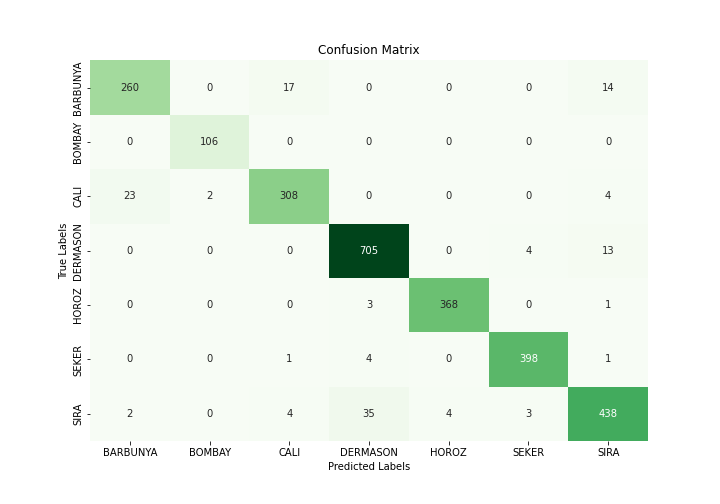
\includegraphics[scale=0.3]{../Plots/Classification tree confusion matrix.png}}
%     \caption{Classification tree confusion matrix}
%     \label{clf confusion matrix}
% \end{figure}
Classification Report:
              precision    recall  f1-score   support

    BARBUNYA       0.86      0.91      0.88       289
      BOMBAY       1.00      1.00      1.00        98
        CALI       0.93      0.89      0.91       323
    DERMASON       0.95      0.98      0.97       698
       HOROZ       0.99      0.99      0.99       383
       SEKER       0.99      0.99      0.99       391
        SIRA       0.97      0.92      0.95       536

    accuracy                           0.96      2718
   macro avg       0.96      0.96      0.96      2718
weighted avg       0.96      0.96      0.96      2718

\end{document}